\usepackage{tikz}
\usetikzlibrary{calc,shapes,decorations.markings}
\usepgflibrary{shapes.geometric}

% Syntax: \Cylinder{<x-coordinate>}{<y-coordinate>}{<name>}{<shownName>}
\newcommand\drawOsdCylinder[4]{%
\tikzset{Cylin/.style={cylinder, shape border rotate = 90, draw, cylinder uses custom fill,
cylinder end fill = blue!20, cylinder body fill = blue!20, minimum height =2cm,
minimum width = 1.5cm, opacity = 1, aspect = 0.5}}
\node[Cylin] (#3) at (#1,#2) {#4};
}

\newcommand\drawMdsCube[2] {
\coordinate(p) at (#1,#2);
\draw[fill = red!20] ($ (p) + (-1,0.5) $) -- ($ (p) + (-0.75,0.75) $) -- ($ (p) + (1.25, 0.75)$) -- ($ (p) + (1, 0.5) $);
\draw[fill = red!20] ($ (p) + (1.25, 0.75)$) -- ($ (p) + (1.25, -0.25) $) -- ($ (p) + (1, -0.5) $) -- ($ (p) + (1, 0.5) $);
\node[rectangle, draw, fill = red!20, minimum width=2cm, minimum height=1cm] () at (#1,#2) {MDS};
}

\newcommand\drawClientCircle[2] {
\coordinate(p) at (#1, #2);
\node[circle, draw, fill = green!20, minimum width=2cm] at ($ (p)+(0.2,0.2) $) {};
\node[circle, draw, fill = green!20, minimum width=2cm] at ($ (p)+(0.1,0.1) $) {};
\node[circle, draw, fill = green!20, minimum width=2cm] at (p) {CLIENTS};
}

\newcommand\drawMonitorDiamond[2] {
\node[diamond, draw, fill = yellow!20, minimum width=1.5cm, minimum height =
1.5cm] () at (#1, #2) {MONITOR};
}
\newcommand\drawArch{
\begin{figure}[!h]
	\begin{center}
		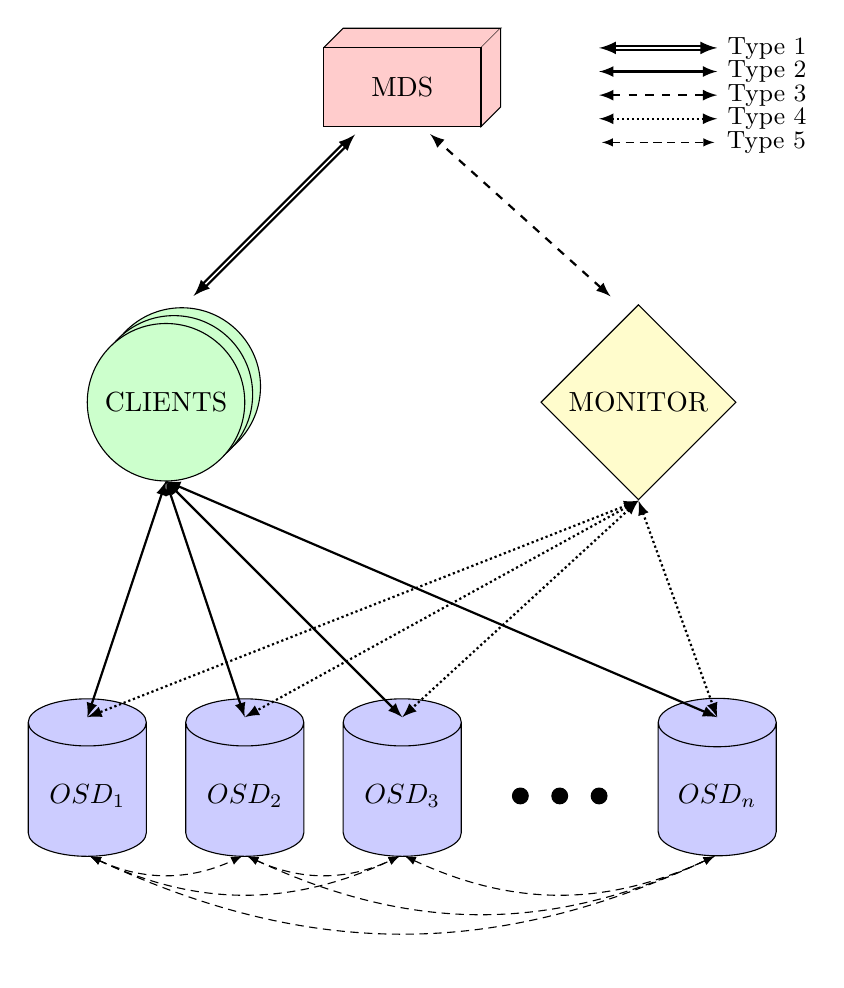
\begin{tikzpicture}[
			t5/.style={thin,<->, densely dashed,bend right=25, shorten >=1pt,shorten <=1pt,>=latex},
			t1/.style={thick,<->,double, shorten >=4pt,shorten <=4pt,>=latex},
			tt1/.style={thick,<->,double, shorten >=0pt,shorten <=0pt,>=latex},
			t2/.style={thick,<->,shorten >=0pt,shorten <=0pt,>=latex},
			t3/.style={thick,<->, dashed, shorten >=4pt,shorten <=4pt,>=latex},
			tt3/.style={thick,<->, dashed, shorten >=0pt,shorten <=0pt,>=latex},
			t4/.style={thick,densely dotted,<->,shorten >=0pt,shorten <=0pt,>=latex}]

			%\whitebodyCylinder{0}{0}{}
			%\draw[help lines] (0,0) grid (10, 10);
			% drawing OSDs
			\drawOsdCylinder{1}{0}{osd1}{$OSD_1$} \drawOsdCylinder{3}{0}{osd2}{$OSD_2$}
			\drawOsdCylinder{5}{0}{osd3}{$OSD_3$}
			\filldraw[black] (6.5,0) circle(0.1);
			\filldraw[black] (7,0) circle(0.1);
			\filldraw[black] (7.5,0) circle(0.1);
			\drawOsdCylinder{9}{0}{osdn}{$OSD_n$}

			% drawing MDS
			\drawMdsCube{5}{9}

			% drawing Clients
			\drawClientCircle{2}{5}

			% drawing Monitor
			\drawMonitorDiamond{8}{5}

			% drawing arrow
			\draw[t1] (2.25, 6.25) -- (4.5, 8.5) {};

			\draw[t2] (2,4) -- (1, 1) {};
			\draw[t2] (2,4) -- (3, 1) {};
			\draw[t2] (2,4) -- (5, 1) {};
			\draw[t2] (2,4) -- (9, 1) {};

			\draw[t3] (7.75,6.25) -- (5.25,8.5) {};

			\draw[t4] (8,3.75) -- (1,1) {};
			\draw[t4] (8,3.75) -- (3,1) {};
			\draw[t4] (8,3.75) -- (5,1) {};
			\draw[t4] (8,3.75) -- (9,1) {};

			% sample arrow
			\draw[tt1] (7.5,9.5) -- (9,9.5) node[right, right] {\small{Type 1}};
			\draw[t2] (7.5,9.2) -- (9,9.2) node[right, right] {\small{Type 2}};
			\draw[tt3] (7.5,8.9) -- (9,8.9) node[right, right] {\small{Type 3}};
			\draw[t4] (7.5,8.6) -- (9,8.6) node[right, right] {\small{Type 4}};
			\draw[t5] (7.5,8.3) -- (9,8.3) node[right, right] {\small{Type 5}};

			\draw[t5] (1,-0.75) to (3, -0.75) {};
			\draw[t5] (1,-0.75) to (5, -0.75) {};
			\draw[t5] (1,-0.75) to (9, -0.75) {};
			\draw[t5] (3,-0.75) to (5, -0.75) {};
			\draw[t5] (3,-0.75) to (9, -0.75) {};
			\draw[t5] (5,-0.75) to (9, -0.75) {};

		\end{tikzpicture}
	\end{center}
	\label{arch}
	\caption{Architecture of NCVFS}
\end{figure}
}
